\documentclass[twocolumn, 11pt]{IEEEtran}
\usepackage{blindtext, graphicx}
% *** CITATION PACKAGES ***
%
\usepackage{cite}
% correct bad hyphenation here
%\hyphenation{op-tical net-works semi-conduc-tor}
\usepackage{algorithmic}
\usepackage{multirow}
\usepackage[options ]{algorithm2e}

\begin{document}
%
% paper title
\title{\vspace{-0.5in} WALE: A Weighted Adaptive Location Estimation Algorithm}
\author{Darshak Sundar, Siddharth Sendil, Vasanth Subramanian\\ and Vidhya Balasubramanian \\Department of Computer Science and Engineering\\Amrita School of Engineering, Coimbatore\\ Amrita Vishwa Vidyapeetham (University), India}
\maketitle


\begin{abstract}

%\boldmath
Indoor Localization using Wi-Fi is gaining ubiquitous usage owing to its simplicity and inexpensiveness. A conventional method of localization is trilateration which can be accomplished using signal strength or time of flight of a radio signal between receiver and transmitter. However trilateration is prone to errors in accuracy which can occur due to various factors. Commonly, a reason for the failure of trilateration is due to the errors in distance estimation which makes the quality of trilateration poor. In this paper, we propose a novel  Weighted Adaptive Location Estimation (WALE) algorithm. The proposed algorithm improves the accuracy of localization over the basic trilateration by taking into account the quality and properties of the circle overlaps in the trilateration region. Based on the overlap properties a distance re-estimation, and a classification of points, based on whether they are trilaterable, is performed. A maximum likelihood estimation over a weighted grid of this region based on an exponential distribution provides the location estimate. Our experiments over real indoor testbeds have demonstrated that our algorithm provides much improved accuracies without fingerprinting both in the average and worst case. 
\end{abstract}
\footnotetext{This work has been funded in part by DST(India) grant DyNo. 100/IFD/2764/2012-2013} 
%\IEEEpeerreviewmaketitle

\section{Introduction}
Indoor Localization and tracking has become ubiquitous in these days of smart spaces and smart environments. ... [Applications] ... Under smart phone localization, even though lots of sensors, bluetooth and other technologies being used aid in position estimation, Wi-Fi is is predominant when it comes to localization. In this paper, our focus is improving accuracy of Wi-Fi localization. Since Wi-Fi is the most common approach to localization, our method plays a major role in improving performance of localization in Wi-Fi so that the overall accuracy is improved.

Wi-Fi localization works based on received signal which consists of various parameters including Received Signal Strength Indicator (RSSI), Angle of Arrival (AoA), Time of Arrival (ToA) and Channel State Information (CSI). In general, CSI, ToA and AoA require specialized equipment or chipsets and proper time synchronization, which make the adoption for common use difficult. RSSI, however can be easily measured in standard smartphones and it is more commonly used for localization, despite its inaccuracies \cite{RSSI Analysis}. Localization techniques that use RSSI commonly uses fingerprint maps which takes huge effort and immense time to generate. However these techniques provide the best accuracies when using WiFi as the primary technology \cite{microsoft competition}. While there are a few non-fingerprinting approaches that use RSSI as the base parameter, they suffer from poor accuracies. The labour involved in fingerprinting techniques and the low reliability offered by non-fingerprinting techniques open up avenues for further research in developing better and robust non-fingerprinting localization algorithms.

In this context, least-square based approach and multilateration are the most well known non-fingerprinting methods for localization that use RSSI. In the least square  method, difference between $N$ equations of circles with $(N-1)$th circle equation are calculated. The solution is the value with minimum of sum of squares. These methods require 4 or more access points for estimation and is more complex. Multilateration helps in estimating a relative or an absolute point among $k$ spheres or circles (in 2D) whose radius is the estimated distance from the access points. In multilateration, two access points are considered at a time and infinite number of points are marked between them. From each beacon hyperbolic curves are plotted along the marked points. The intersection points provides an estimated location. Since multilateration is complex, trilateration is most commonly used.

In trilateration since the intersection region is primarily dependent on the radii of the three circles, which in turn is dependent on a distance estimator using  RSSI, the accuracy of position estimate is affected by the accuracy of the distance estimation method. Distance estimation methods use path-loss models like log-distance model, ... to calculate distance based on RSSI. However the estimated distance is inaccurate since these models do not adequately account for obstacles inside the indoor space, dispersion, reflections etc. In order to reduce the error in trilateration, one option is to define a better propagation model. This may be developed for specific environments, but is not generalizable, and cannot account for people movement and other dynamic factors that may affect RSSI.

In Trilateration, it is observed that more often than not, the circles do not intersect. It is also observed that one of the circles may completely enclose another. This is caused either due to more signal strength loss than initially predicted or due to the presence of certain objects in the environment that make the data inconsistent, which are unavoidable in either case. As a result of this, we design our approach based on two key ideas: One, due to errors in distance estimation, we classify a point into two categories; one where trilateration can be applied and one where it fails. The other, that based on distance estimation the likelihood of a point lying towards the outer regions of the circle are higher. Reinforcement of this despite trilateration errors is essential. To account for the former a classification of points based on trilaterability is done. To account for the latter, we model the region of interest as a weighted grid, where the weights follow an exponential curve, and this closely follows the log-distance model. Weighting in the common regions is based on the trilaterability. A maximum likelihood estimation over this weighted grid of this region provides the location estimate.


%WiFi localization operates by locating a WiFi receiver

%The cost of fingerprinting techniques, and the poor accuracies of non-fingerprinting RSSI based techniques

%Now talk of trilateration and least square approaches, and why it is essential to look at it. Then explain the issues of the same..then state understanding the environmental causes or modeling it is impossible. We look at the trilateration itself to find clues..

%then give overview of our approach...We based our approach based on two key ideas: One is that, due to errors in distance estimation, the approach trilateration itself does not work for some points i.e the point is not in the overlapping region of three circles, therefore based on the circles we classify a point into two categories, one where trilateration can be applied and one where it fails...next, the probability of the point lying in a fuzzy band near the border of the circle is higher than the center..there is a reference for it. By considering the log-distance propagation itself, we come up with an approach that does a weighted adaptation (need to provide a more clearer and meaningful name).. to basic trilateration where weights are a function of the radius and follows a logarithmic curve. This approach is modified according to the class of the point. ....


 

 
\section{Related Work}


%Most of the RSSI based systems, operate upon on either of the two major variables: Time or Distance. Time based localization \cite{TOA} techniques rely upon either specific hardware \cite{TDOA}, information extracted from channel state information or make essential assumptions about the area. Techniques reliant upon distance use propagation models to better map the RSSI to a distance and then perform multi-laterations to accurately localize the area.  Trilateration while easier to implement has very low accuracy owing to the lack of perfect distance propagation models. Hence fingerprinting is often clubbed together with the multilateration techniques. But its dependency on radio-maps, which have proved to be laborious and time-consuming, is also fickle due to its reliance on the environment. Algorithms such as \cite{DCE} proposed, aim to improve accuracy but they fail due to the poor stability of the 2.4 GHz band. 


%WiFi localization techniques fall into numerous categories. Several location estimation techniques attempt to model signal propagation through space \cite{radar}, assuming known locations of access points and an exponential signal attenuation model. However, even when taking into account furniture and walls of different material the accuracy is limited. There are other techniques that attempt to localise using RSSI fingerprint data using a Markov model, kNN based approach, for example \cite{RSSI} focused on baby tracking in an indoor environment which proved to be effective, however, it will become onerous when shifting to an unknown location. While more accurate than signal propagation models, these methods are inherently discrete and have only limited capabilities for interpolation between locations.

%Wireless Sensor network need to establish links between them for initial connections. Previously this was done using snooping or flooding  techniques. Now an RSSI based approach \cite{Under} is being used because establishing these links in an unsymmetrical environment yields unsolicited results. Also in a WSN approach \cite{Analysis_RSSI}, uses database switching as per the position of reference node need to be done. This helps in switching from indoor to outdoor environments, but requires complete knowledge of the area, otherwise error percentage will increase. Other experiments \cite{Zhang15} showed that although the accuracy of RSSI received at a single antennae is highly fluctuating, a Feature Vector which is formed by lots of RSSI values from different APs is a certain stability. This algorithm was able to obtain accuracies ranging between 2m-4m. However, to obtain this Feature Vector the localisation region is divided into grids which requires extensive work to implement. Moreover, after obtaining the Feature Vectors in real-time, they are compared to existing Fingerprinted Feature Vectors to obtain this accuracy.

%Systems such as \cite{radar}, uses signal strength and signal to noise ratio along with triangulation, Ekahau \cite{ekahau}, in addition to signal strength requires extensive site surveying to calibrate the underlying localization system, while accurate are expensive to implement and time-consuming. \cite{ekahau} also uses signal strength but in addition it requires a site survey to calibrate the system and WiFi location tags to be present on the user. These IPSs are susceptible to several factors that affect the RSSI and hence subsequently reduce their accuracies. COMPASS \cite{compass} takes the orientation of the user into account but it also is reliant on an elaborate fingerprint of the target area which is laborious. There are also a multitude of systems that are hybrid variants and use various other technologies such as Bluetooth, RFID, Infrared in addition to WiFi.  Perez et al. \cite{fusion} propose a system where trilateration is performed using the signal strength of the Bluetooth waves and then an approximate localized region is obtained. Techniques such as these inculcate specialized hardware which makes them expensive to deploy and test. Hence our aim is to minimize the cost and develop a system that works with the existing infrastructure. In this paper, we devise an approach that aims to solve the aforementioned issues by suggesting a cost effective method that doesn't compromise on the precision of localization. 

 %Although the latent potential of such a system has been theorized, a solution that address accuracy, reliability, scalability and cost-effectiveness has not yet been proposed.  


%talk more about inertial sensors
%talk more about other papers - 
%talk more about fingeprinting 
%talk more about survey papers
%cluster the papers together
Recently, Indoor positioning has garnered widespread interest from various communities because of the sheer number of applications it has and the myriad of problems it solves.
There are several proposed systems that bring about high accuracy up to a few centimeters. 
Methods such as Bat \cite{barshan1992bat}, Cricket \cite{priyantha2000cricket} rely on a mixture of Radio and Sound signals to perform indoor positioning. Active badge \cite{want1992active} uses infrared IR beacons and receivers for location sensing. 
Well known methods such as Landmarc \cite{ni2004landmarc} and SpotON \cite{ hightower2000spoton} use active RFID tags to perform location sensing. \cite{ni2004landmarc} achieves an average error of 1m. But inadvertently all of these techniques facilitate the use of specialized infrastructure which is unequivocally expensive and convoluted.

A method to alleviate this dependence on special infrastructure sparked the use of RF signal maps (fingerprints) of the target area \cite{kaemarungsi2012analysis, kaemarungsi2004RSSIproperties, badawy2007RSSidecision, zhang15}. 
Fingerprints contain the RSS measurement of RSS transmitters whose position is known in each location and localization is performed by matching the observed RSS with the database. 
RADAR \cite{bahl2000radar} was one of the first systems that utilized the signal intensity of RF waves for indoor positioning. RADAR uses a deterministc fingerprint for each location. 
Recently, there have been methods presented that use other factors in addition to RSS to increase the dimensionality of RSS dependent fingerprints. SurroundSense \cite{azizyan2009surroundsense} in addition to RSS, uses other attributes such as ambient sound, light, color etc. 
Evidently, fingerprinting requires laborious effort, is extremely time consuming and the map has to be updated constantly due to being vulnerable to changes in the environment. 
To mitigate this hurdle, \cite{ledlie2012mole} uses a dynamic user generated fingerprint that is intelligently updated over time. 
\cite{yin2008LEMT} accounts for the variations in the RSS in fingerprints due to environmental factors by using model trees to reconstruct the radio map in real time. 
Ekahau Inc \cite{ekahau}, offers a commercial positioning system which boasts very high accuracy of 1m but it requires extensive site surveying. 
Techniques to better the mapping methods were developed to eliminate the need for fingerprinting such as DAIR. But it presumes a dense network of APs than commonly available. 

Other sensor based approaches \cite{li2012Intertial1, qian2013Intertial2} use inertial sensors in smartphones in addition to RSS to perform localization. While they achieve a higher precision, dependence on specialized hardware decreases the cost effectiveness.
Lateration based techniques which determine the position of the device are dependent on the distance measurement from nearby beacons \cite{farid2013recent} .  Trilateration requires ranging techniques for distance measurement between nodes such as Time of Arrival (ToA) \cite{TOA}, Angle of Arrival (AoA) \cite{AOA}, Time Difference of Arrival (TDoA) and RSSI \cite{roxin2007survey}.  
\cite{li2000comparison, yamasaki2005tdoa, TDOA} use TDoA based approaches using WiFi to perform localization. While \cite{yamasaki2005tdoa} claims a mean accuracy of 2.4m, TDoA based localization is not feasible in typical WiFi hardware because of its dependence on acute time synchronization. Hence,
RSSI is more commonly used because it’s unconstrained by the hardware. RSS \cite{RSSI_Analysis,Analysis_RSSI} based localization  is coupled with RF propagation models and lateration techniques. These propagation models estimate the distance by aiming to account for the signal losses in the environment. However these models are not accurate enough to perform trilateration on their own. \cite{DCE} implements an algorithm that accounts for this divergence.

In our paper, we propose a method that is a RSSI based weighted adaptive trilateration localization algorithm that uses distance estimation models to accurately localize nodes. Section 3 highlights the analysis of trilateration being performed on our dataset and the problems that occurred. In section 4 we describe our algorithm and discuss the results in section 5. 

    

\section{Analysis of Trilateration}


As discussed in previous sections it is important to develop non-fingerprinting based solutions for indoor localization. Additionally, such solutions should preferably work with signal-strength information since they do not require additional hardware. Trilateration is a basic non-fingerprinting approach, which is robust and easy to implement but suffers from poor accuracy. However there is scope to adapt and improve trilateration. Towards this we have analyzed the performance and patterns in trilateration and identified the potential areas for improvement and this section goes into the details of this analysis. 

Firstly we discuss the target environment where we conducted our experiments to analyze the performance of trilateration. The target environment is a typical office space with several cubicles and pathways for walking which is analogous to normal indoor settings. Belkin N600 DB Wireless Dual Band N+ Routers were used to collect the dataset. To achieve the optimal coverage of the area, four routers are strategically placed such that the variance amongst them is maximum \cite{kaemarungsi2012analysis , CiscoLocation}. Additionally, the router's relative position from the ground also plays a pivotal role. The RSSI variance between routers influences the optimal positioning, and after analysis \cite{shanmugaapriyan2014pragmatic} , it was observed that for any point, for precise localization, three routers at a maximum distance of 18 m away from each other were required. To eliminate any shadowing due to obstacles, the routers were placed up high ( 2.43m ) \cite{shanmugaapriyan2014pragmatic}, which also aids in maintaining a line of sight with minimum path loss at each point. Thus the routers were positioned as shown in \ref{fig:tenv}.   

%Firstly we discuss the two target environments where we conducted our experiments to analyze the performance of trilateration. The first environment is a typical office space with several cubicles and pathways for walking which is analogous to normal indoor settings. Belkin N600 DB Wireless Dual Band N+ Routers were used to collect the dataset. To achieve the optimal coverage of the area, four routers are strategically placed such that the variance amongst them is maximum \cite{kaemarungsi2012analysis , CiscoLocation}. Additionally, the router's relative position from the ground also plays a pivotal role. The RSSI variance between routers influences the optimal positioning, and after analysis \cite{shanmugaapriyan2014pragmatic} , it was observed that for any point , for precise localization, three routers at a maximum distance of 18 m away from each other were required. To eliminate any shadowing due to obstacles, the routers were placed up high ( 2.43m ) \cite{shanmugaapriyan2014pragmatic}, which also aids in maintaining a line of sight with minimum path loss at each point. Thus the routers were positioned as shown in \ref{fig:tenv}.

% The second target 

\begin{figure}[h]
\centering
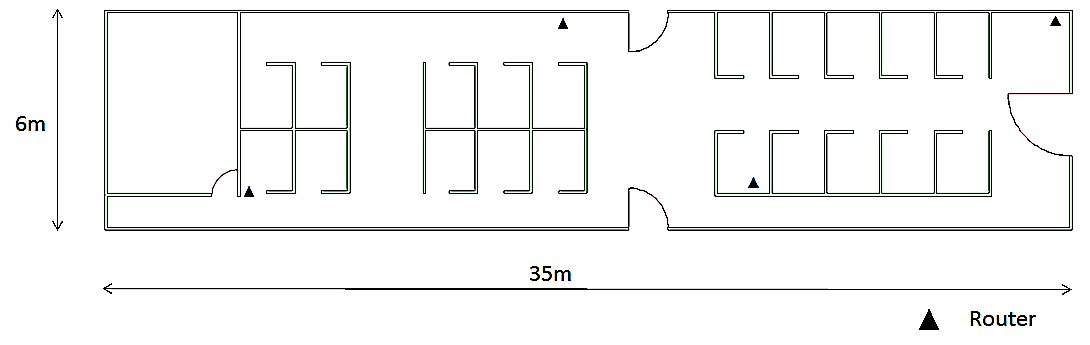
\includegraphics[width=80mm]{Tenv.png}
\caption{Images/Localization area }
\label{fig:tenv}
\end{figure}

Several experiments were conducted in this environment, primarily for fingerprint data collection over several iterations and for localization experiments \cite{shanmugaapriyan2014pragmatic}. Additionally experiments were performed to understand the path-loss in different environments. Our analysis of the trilateration has been conducted over several of these experiment data sets. We first performed trilateration over several points in the fingerprint databases and calculated the overall accuracy \cite{shanmugaapriyan2014pragmatic}. On probing the results, we find that for the majority of the points the intersection region was inaccurate. Hence we used non linear least square regression to better find the probable region, which is a method to approximate the modelling region to a linear one and refine it in succeeding iterations. In this environment, We noted an average accuracy of 7.76m with it being .64m in the best case and a terrible 21.49m in the worse case scenario. 
The accuracy definitely needs to be improved, therefore warranting further analysis. Upon further examination, it was discerned that the source of this discrepancy could be attributed to the error in distance estimation. Distance estimation is based on appropriate distance propagation models.
%Sid said he'd give me the accuracy asap for this. 

%*******************************
%We observed that the average error in our environment is ... , maximum error is .... and minimum is ...

%It was discovered that due to the poor accuracy of the propagation model, trilateration by itself fails. We observe that a major factor affecting the accuracy of trilateration is the distance estimation method.

%DO NOT DELETEEEEEEEEEEEEEEEEEEEEE- outline for section
%tell impact of these models and how it affects accuracy. ..however while this underestimation and overestimation can be attributed to different environmental factors, it is difficult to account to for it and correct it without knowing the environment fully. So we look at the geometric properties of circles to see whether these problems can be identified. Additionally we determine other contributing factors for ....

% From our analysis we see the following
% 1. The underestimation and overestimation can be observed from the circle overlaps...
% 2. There are cases for which trilateration will not work..explain using examples...
% 2. The probability of a point lying towards the border of a circle is higher than being in the center. 

%In our paper we use these insights to develop a WALE algorithm that combines a probabilistic weighting approach with a dynamic circle resizing approach. The approach is customized based on whether a point is trilaterable or not. The next section will explain this algo in detail. 

%*******************************

%There are several propagation models that exist. Models such as Hata, Log distance path loss, ITU and Okamura, dependent on the log-distance equation to model the signal pathloss, are widely accepted due to their derivation from the Free space path loss model [ 2 ] , which results from the inverse square law and the antenna gain. For our experiments, we consider the Log Distance Path loss model, an extension of the Friis free space model, as our RF propagation model \cite{sarkar2003survey, soorty2015finding}
There are several propagation models that exist. Models such as Hata-Okamura, Log distance path loss, ITU etc. are dependent on the log-distance equation to model the signal path loss. These models are widely accepted due to being derivations of the Free space path loss model, which originates from the inverse square law and the antenna gain. For our experiments, We consider the log distance path loss model as our RF propagation model \cite{sarkar2003survey, soorty2015finding}.

\begin{equation}
\Bigg[\frac{P_{L}(d)}{P_{L}(d_{0})}\Bigg]_{dB}  ~=~ -10n log\Bigg(\frac{d}{d_{0}}\Bigg) + X_{dB}
\label{pathlosseqn}
\end{equation}
Where:

\begin{itemize}
 \item PL(d0) is the total path loss measured in (dB) at a distance d0.

\item PL(d) is the total path loss measured in (dB) at the distance d1.

\item 'n' is the path loss exponent. which has been empirically found out to be 3 in our case. 

\item 'X' is a zero mean Gaussian distributed random variable (in dB) with standard deviation \( \sigma \). Since the shadowing effect in our experiments is inconspicuous and can be ignored, 'X' is equated to 0
 
\end{itemize}
%While environmental factors cause the errors in trilateration, our goal is to identify the effects on trilateration and not analyze the cause i.e, we only look at the geometric patterns of the circles and their impact on the accuracy.  
%insert our graphs here - 
%add a para about the issues in path loss models . 

While the log distance path loss model takes shadowing into account, it still is founded upon empirically derived evidence and does not hold good in all environments. The path loss exponent is an important parameter and not choosing an appropriate value could considerably alter the end results \cite{srinivasa2009path}. Furthermore, the path loss exponent is prone to change with changes to the environment and is also affected by the obstacle density in room. In the case of an empty building, the value of the path loss exponent would shift towards the lower end of the spectrum. In such a case, the distance being estimated would be much lower than the one in in heavily dense environments, such as a file/stock room, where it would lean towards the higher end. In addition to this, the power of the signal drops when passing through walls. Thus in an office like environment where there are several partitions, the possibility of the signal attenuating is high and this may translate into a high RSS due to a weaker signal and consequently a large distance being estimated even though the actual distance is low. Thus the dependence of the path loss exponent on environmental factors coupled with the variable nature of RSS evidences the fickleness of propagation models. 

Our goal here is to identify the ramifications of these factors on trilateration and methods to alleviate the error, and not the factors themselves. For this, we look at the geometric patterns of the circles and their impact on the accuracy. Taking that into consideration, we look into the overlapping region of the circles. It was observed that two major reasons contributing to the failure of trilateration due to an unfavourable overlapping region were underestimation and overestimation. 

%While environmental factors cause the errors in trilateration, our goal is to identify the effects on trilateration and not analyze the cause i.e, we only look at the geometric patterns of the circles and their impact on the accuracy. Taking that into consideration, we look into the overlapping region of the circles. Two major reasons contributing to the failure were underestimation and overestimation. 
 

 %\item Underestimation
 \begin{figure}[ht!]
\centering
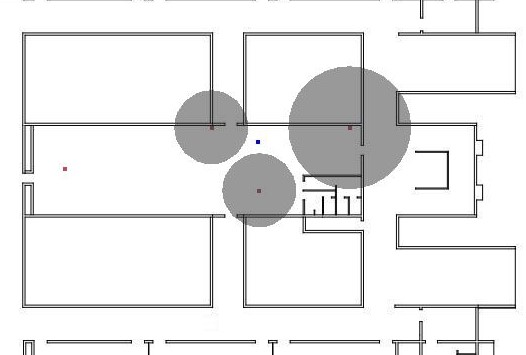
\includegraphics[width=80mm]{Images/Underestimation.jpg}
\caption{ Images/Practical Example of Underestimation \label{overflow}}
\end{figure}

 
Underestimation occurs when the circles do not intersect each other in a manner to distinctly find a common region among them. It can be observed in either of these probable possibilities viz. three completely non intersecting circles, one circle intersecting with two others and only two circles intersecting. Hence localization becomes inherently improbable as there is no common region between the three circles to leverage out a point to accurately depict the actual position of the device. After the evaluation of trilateration in our data-set, underestimation in one form or the other occurred in around 57\% (48 instances) of the cases. 
 
%encompassing definition  ; 2 paragraphs; formalism; analysis in our cases % of cases; add example diagram ;


%\item Overestimation 
\begin{figure}[ht!]
\centering
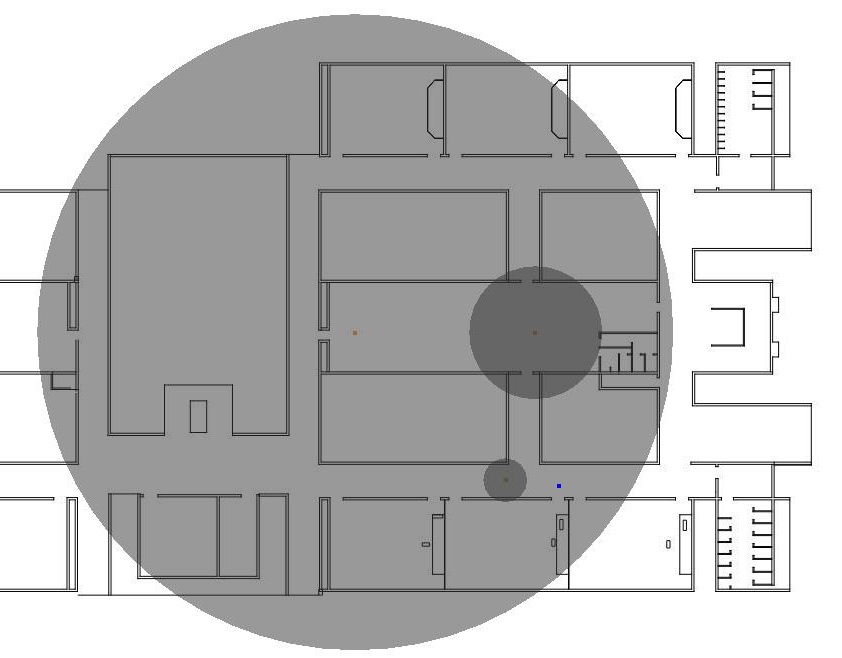
\includegraphics[width=80mm]{Overestimation.jpg}
\caption{ Images/Practical Example of Overestimation\label{overflow}}
\end{figure}

Conversely, Overestimation occurs when one circle completely encompasses the other circle(s). In such cases, the intersecting region is a large ambiguous area where localization becomes improbable. Typically, when the intersecting region is large its centroid is considered to be estimated point. But in such cases, this becomes meaningless as the centroid lies near the centre of the larger circle. %Overestimation accounted for xx\% of the cases in the second environment. 

%\{figure}[ht!]
%\centering
%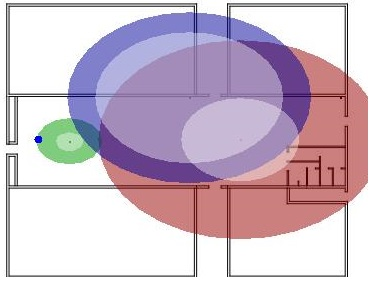
\includegraphics[width=80mm]{log(1,3).jpg}
%\caption{ Practical Overestimation Example \label{overflow}}
%\end{figure}

\begin{figure}[ht!]
\centering
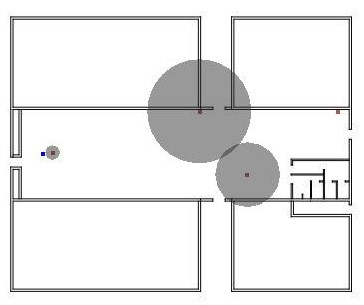
\includegraphics[width=80mm]{strongpoint.jpg}
\caption{ Images/Device close to a router \label{overflow}}
\end{figure}

%It was also observed that for a number of instances in underestimation, when the location of the device was in close proximity to one of the routers, the position of the device was always within the region of the smallest circle.
%Upon further analysis, it was observed that when the location of the device was in close proximity to one of the routers, its position was always within the region of the smallest circle. 

It was also observed that when the radius of the second smallest circle exceeded that of the smallest by a factor of \(\beta\) the position of the device was in close proximity to one of the routers and laid near the outer regions of the smallest circle. 43\% of the instances in the dataset conformed to this observation.  

% From figure(2) we can see that when one or more of circles depicts a much larger radius than theoretically predicted, we may call it overestimation.The problem with both is that it is unclear whether we can definitively categorize based on the smaller or bigger sizes of the circles. This issue still needs to be addressed, but this paper offers a method that can be considered.
 
Thus to alleviate this flaw, A recalibration of the estimated distance would result in better localization. This recalibration could be achieved by either systematically increasing the radii of the three circles till they intersect or by decreasing them till the intersection region is meaningful \cite{DCE}. In cases of close proximity, it could be discerned that the likelihood of the device existing near the circumference was higher than it lying near the center. Hence, the overall system could be bifurcated into major sections; One requiring trilateration and the other not.


%To summarize the following are the major insights based on our analysis, and our proposed algorithm is based on these findings.
%From our analysis we perceive the following
% 1. The underestimation and overestimation can be observed from the circle overlaps...
% 2. There are cases for which trilateration will not work..explain using examples...
% 2. The probability of a point lying towards the border of a circle is higher than being in the center. 

To summarize, the following are the major insights based on our research:
\begin{itemize}
    \item The underestimation and the overestimation of the intersection region in trilateration can be observed from the circle overlaps.
    \item There are cases when trilateration doesn't apply. Instances when the radii of the smallest circles exceeds that of the middle circle by a factor of \(\beta\), the actual point was observed to be in close proximity to one of the routers. 
    \item In the above case, it was gleaned from the data that the actual point laid in the outer region of the circle more often than in the central regions. 
\end{itemize}

%We primarily test out two algorithms that aim at solving this issue. We then propose our own algorithm and improve the results.

%We test out two algorithms that aim to solve this issue: The first one increasing the radii by a constant 10 percent of the original value and the second one being Dynamic Circle Expansion \cite{asd}. We propose a method that is an improved adaptive version of the two algorithms stated.

In our paper we use these findings to propose WALE (Weighted Adaptive Location Estimation), an algorithm that combines a probabilistic weighting approach with a dynamic circle resizing approach. The approach is customized based on whether a point is trilaterable or not. The next section will explain our algorithm in detail. 


\section{Weighted Adaptive Location Estimation }

In this section we describe our approach to improve the indoor localization without fingerprinting by designing a Weighted Adaptive Location Estimation Algorithm based on an initial trilateration. This approach is based on three major aspects:
\begin{itemize}
\item Determining whether the distance estimation from the routers has been underestimated or overestimated based on the trilateration pattern and accounting for it. 

\item Identifying whether trilateration is feasible for a given location estimation or not

\item Using a novel weighting function that assigns weights with higher probability to points nearer the re-estimated boundary of a disc, and lowest probability towards the center. 
\end{itemize}

Based on this the overall outline of our approach is as follows. For a given point, the distances to the three nearest routers are estimated using the log-distance model. The distances also provide an indication of the type of overlap of the three circles in trilateration and thereby the quality of trilateration. This gives us an idea if the distance is underestimated or overestimated per router. We develop a novel distance re-estimation algorithm which modifies the radii of the circles. Then based on the ratio of the original distances the points are classified as whether they can be trilaterated or not.  A weighting function is applied across the radius of the circle to estimate the probability of a point lying at any potential distance from the center. Using this function, and the classification we come up with an algorithm that calculates the maximum likelihood position. 

\subsection{Distance Re-estimation}

The RSSI signals received from the routers is used to calculate the distances based on the log-distance model. However, the calculated distances may not be perfect, and this may result in the circles either not intersecting at all or circles encompassing other circles as discussed previously. This results in errors in estimating the position, and therefore a re-estimation of the radii of the three circles becomes necessary. There have been attempts to develop circle expansion algorithms to improve trilateration like the Dynamic Circle Expansion (DCE) algorithm \cite{DCE}. The DCE works by fixing the smallest circle, and expanding the other two, based on the ratios of their signal strengths. However this assumes that the highest RSSI reading can be trusted always, which is not always the case, it could also be a case of underestimation. Additionally the DCE does not consider overestimation cases, so it is only a cyclic increase algorithm. Therefore we design a Cyclic Distance Re-estimation algorithm that resizes the circles either by increasing or decreasing the radii as needed. It works on the following principles: 1) when RSSI is strong it is likely to be right, so resizing should be minimal for that router 2) when two circles are close or nearly intersecting, it should also be considered.

Consider an array of circles $C$, which are sorted in decreasing order of radius, and a queue Q used as a temporary data structure. Each circle $c_i \in C$, it is defined by the original radius $r_i$ and the reestimated radius $r_i'$.  $r_i'$ is same as  $r_i$ initially. The algorithm for resizing the circles is given in \ref{CRalgo}. 

\begin{algorithm}
\SetAlgoLined
\KwResult{Circles with meaningful intersection region}
\While{$C[0].getFlag()==0  OR  C[1].getFlag()==0  OR  C[2].getFlag()==0$}{
$i\leftarrow Q.deQueue()$\;
\If{C[i].isEnclose(C[(i+1) mod 3]) OR C[i].isEnclose(C[(i+2) mod 3])}{
$r_i'$\leftarrow $r_i'$ - \alpha * $r_i$\ \;
Q.enQueue(i)\;
}
\Else{
\If{!(C[i].isOverlap(C[(i+1) mod 3]) AND C[i].isOverlap(C[(i+2) mod 3]))}{
$r_i'$\leftarrow $r_i'$ + \alpha * $r_i$ \ \;
Q.enQueue(i)\;
}
}
\Else{
C[i].setFlag(1) \ \;
Q.enQueue(i)\;
}
}
\caption{Algorithm for Distance Estimation}
\label{CRalgo}
\end{algorithm}

The algorithm works as follows. The algorithm starts with the largest circle. The radius of the circle is compared with that of the next two circles. If one of the circles encompass another, then the radius of the encompassing circle gets decreased by $\alpha$ percentage of the radius. If the circle overlaps with other two circles, then no further increase or decrease to radius will happen to the circle. If the circle does not intersect with both of the two circles, then the radius will be increased by $\alpha$ percentage of the radius. The above steps are repeated for the next larger circle and then the smallest circle. This increase takes place in a cyclic manner to all three radii until all the circles overlap with each other without too much overlap. Here $\alpha$ is set experimentally. 

%<Image of both cases at same point for DCE and our algo.. Show our algo works much better than DCE> 



%Our algorithm considers the approach of both the mentioned cases. A simple incrementing algorithm or DCE algorithm, when used for re-estimation, stops incrementing once it finds an overlap with a circle. There could be certain points which does not give a proper distance estimation even after applying re-estimation algorithm. In order to overcome these errors, our algorithm goes for further classification of points in cases where trilateration fails to estimate the distances.

%@@@@@@@@@@@@@@@@@@@@@@@@@

%Explain how we say under-or over-estimation based on the circle overlaps or lack of it. Then our algorithm followed by brief explanation..
%Justification for why cyclic..we need to say two aspects influence - 1)when rssi is strong it is more likely to be right, so resizing should be minimal for that router 2) when two circles are close or nearly intersecting, it should also be considered (DCE does this). So we go for an approach that considers both...since it resizes from the largest, but once overlapped we dont continue increasing..Some justification/examples to say why choosing one of the two alone wont be sufficient.


\subsection{Classification of Location Points}

Before estimating the position we classify each candidate point $p$ as trilaterable or not based on the ratio of the original radii. The ratio of the smallest circle to the next larger one is checked and if it is less than $\alpha$, then this point will not lie in any overlapping region of the circles even after re-estimation, therefore not trilaterable. An example of this case is shown in the \ref{dce_fail}. Whenever the router has a strong RSSI and there is a combination of underestimation and overestimation, the estimated point will never lie in an overlapping region even after re-estimation. In this case, trilateration will yield a huge error in estimating distance. We come up with a novel weighted-solution for this case and it proves to give a much better accuracy in distance estimation.
 
To estimate $\alpha$ a sample set of points from a region are taken, and their distance to the closest three routers estimated. The ratios are calculated and the median of the frequency distribution of these ratios gives a potential estimate for $\alpha$. We have found that this works reasonably well for different environments. However $\alpha$ can also be determined experimentally and fine tuned. 


%<Image of New Method Accuracy working better than DCE>



\subsection{Weighted}

After classifying the candidate point $p$ as above, the location of $p$ is estimated by a novel weighting algorithm which is explained in this section. Firstly, a weighted occupancy grid is overlaid on the region of interest. The weight is calculated for every radius $k$ varying from $0$ to $r_i'$, therefore the weight is uniform for every point along the circumference of a circle with radius $k$.

Weights are calculated for each classified distance using the equation:
\begin{equation}
W[k] = \frac{1}{r}  e^{\frac{k}{r}}    
\end{equation}

The weighting follows the log-normal distribution of RSSI, and gives higher weighting to the points in the border of the circle and lower weights to points closer to the center. 


%#### rewrite
\begin{algorithm}
\SetAlgoLined
\KwResult{Location estimate of device}
\For{$i\leftarrow 0$ $to$ $2$}
{
\For{Each $k\leftarrow 0$ $to$ $r_i'$}{
$k \leftarrow Distance(x,y,C[i].centre())$ \;
$W[k] \leftarrow (1/rad)*(e$ \power $(dist/rad))$ \;
\If{ IsTrilaterable($p$)}{
$p.weight \leftarrow p.weight + W[k]$ \;
}
\Else{
$p.weight \leftarrow p.weight - W[k] $ \;
$p.weight \leftarrow abs(p.weight)$ \;
}
}
}
\label{Algorithm for calculating Weights}
\end{algorithm}

The above weighting is generated for each circle. For the overlapping regions between circles the weights are aggregated if the point is trilaterable, else the absolute difference between them is taken. When a point is trilaterable the overlapping regions are given higher weightage. This is similar to trilateration;  however the weighting helps refine the likelihood area where the point could lie. 
When the candidate point is not trilaterable, it is essential to increase the likelihood of it lying in the smallest circle, while reducing the impact of the other routers. Therefore in the overlapping regions, the weighting is reduced by the taking the absolute difference of the individual weights. By doing this the point is pushed towards the smaller circle and away from the others. 

This algorithm by doing an adaptive weighting takes care of different cases that could occur, and helps improve accuracy.



\section{Analysis and Results}

The two major methods of localization in Wi-Fi environments are fingerprinting and trilateration. Fingerprinting is a more reliable method of localizing than trilateration but, fingerprinting can be a very expensive and time consuming process while trilateration is prone to errors. Using extensive studies and experimental analysis, we have looked at the problems in trilateration to come up with a reliable method of localization. The experiments were also used to compare the performance of other known localization methods under the same circumstances.

In this paper, we deal only with 2.4GHz band Wi-Fi. Two experiments were conducted in environments as described in the (references)figures(). As can be inferred from the figures, the first environment is a typical office setup with the position of routers at key locations so as to improve router utilization. The The second environment has semi-open spaces in between, which could increase the complexity of the environment but nonetheless, provide an intriguing idea of the robustness of the algorithm.


Our algorithm performed very well in the typically office-like setup of environment I. The average accuracy was found to be 3.001m as can be seen from the table(). The comparison of our results to other methods has been discussed in forthcoming sections.

Basic Trilateration:
The Leven-Marquad** algorithm was used to localize points using the distance from routers calculated by RSSI readings and the relative positions of the routers themselves. The results showed that the algorithm does not perform very well in typically congested office environments. It can be observed from the table() that there is a need to address any under or over estimation of distance that may be caused due to such environments. So, trilateration by removing such over and under estimations becomes a priority.

Underestimation-DCE:
Underestimation of distances has been handled by DCE et all. In their method, the router with the best RSSI is trusted ie it's value is not changed at any point, while increasing the distance from other routers by a combination factor of the initial estimate of distances.
Crucially, the method does not increase the router with best RSSI, thereby denying any possibility of the point being away from the best router, which is not the case in practice. This is explained by the figure() .

This lead us to observe that increasing or decreasing the influence of a router should be uniform with respect to the routers. With that in mind, we designed a method of incrementing(or decrementing) the distance of routers from points, which has been explained in detail in the previous section.

Comparing the results of our algorithm to DCE(refer Table ()), we see that DCE performs well in cases where the actual point is very close to a router as evidenced in figure(). DCE fails when the point is considerably in between two routers which is clear in figure(). DCE, while only looking at increasing the distance of point from routers, fails in cases where there can be an overestimation of distance due to various factors. Figure() gives an example of such a case. In such cases, the trilateration itself becomes redundant. In our algorithm, we account for such over estimations by having a distance decrement when it becomes necessary(as in these cases).

Even then, the trilateration was not a big success. On experimental analysis, we found that some points are not meant to be trilaterated like the one in figure().
This meant that there could be a division between all localization points- those that can trilaterate and those that cannot. On further analysis, we saw some patterns that could link all such non-trilaterable points. Every such point was pretty close to a single router while being far away from the other routers, or in other words, could depend solely on one router while being negatively influenced by other routers.
This phenomenon can be judged by looking at the relative estimated distances of the point from each router. The distance from the router which is very close to the point was seen to be much smaller compared to the distances from other routers. Hence, we propose(or hypothesize) that the ratio of the smallest distance from a router to the next smallest distance can be seen as a parameter to decide on the trilaterability of a point. 

The use of such a ratio demands the existence of a threshold which would automatically group points into either classification. Such a threshold, $\alpha$ say, would vary based on the environment, but would be a constant once the environment is identified. We arrived at our value of this $\alpha$ after empirical analysis of our experiment.
The accuracies for different values of $alpha$ are recorded in table().

\begin{center}
\begin{tabular}{ |c|c| } 
\hline
$\alpha$ & Accuracy \\
\hline
0.4  & 3.15 \\
0.45 & 3.11 \\
0.5  & 3.06 \\
0.55 & 3.001 \\
0.6  & 3.19 \\
0.65 & 3.25 \\
0.7  & 3.32  \\
\hline

\end{tabular}
\end{center}




************** *****************

1.  Experimental setup, and experiments performed - two experiment results
2. performance of our algorithm, compared to basic trilateration
3. performance of our algo with different values of alpha
4. dce vs our increment...overall and some key examples...take also for only underestimation examples
5.. some examples for overestimation, underestimation...and average for separate types of points




\begin{tabular}{ |p{3.2cm}|p{1.5cm}|p{2.5cm}|  }
 \hline
 \multicolumn{3}{|c|}{Environment - I} \\
 \hline
  & Basic Trilateration &WALE\\
 \hline
 Avg Accuracy  & Cell 1 & Cell 2\\
 Min Accuracy  & Cell 1 & Cell 2\\
 Max Accuracy  & Cell 1 & Cell 2\\
 Standard Deviation& Cell 1&  Cell 2\\
 \hline
\end{tabular}
\label{tab:BASIC vs WALE}


Table: Basic Trilateration vs WALE
\\
\\

\begin{tabular}{ |p{3.2cm}|p{1cm}|p{2.5cm}|  }
 \hline

 \hline
 Environment - I & DCE &WALE $\alpha = 0.55$\\
 \hline
 Avg Accuracy  & 3.648   & 3.001 \\
 Min Accuracy  & 0.605   & 0.429 \\
 Max Accuracy  & 9.089   & 7.94  \\
 Standard Deviation & 1.958 &  1.695\\
 \hline
 \multicolumn{3}{c}{} \\
 \hline

 \hline
  Environment - II& DCE &WALE  $\alpha = 0.60$\\
 \hline
 Avg Accuracy  & 6.192      & 5.105\\
 Min Accuracy  & 1.417      & 1.052\\
 Max Accuracy  & 16.921     &  13.953\\
 Standard Deviation & 4.641 &  3.621\\
 \hline
\end{tabular}
\label{tab:DCE vs WALE}

Table: DCE vs WALE





\bibliography{wifiref}
\bibliographystyle{ieeetr}



\end{document}


